\documentclass[sn-basic, referee]{sn-jnl}

\usepackage{graphicx}
\usepackage{amsmath,amssymb}
\usepackage{booktabs}
\usepackage[utf8]{inputenc}

\begin{document}

\title[Characters: Shakespeare in Silico]{Characters: Constraining Dramatic Evidence via Stage-Presence Epistemology and Prosodic Scansion in the Shakespeare Corpus}

\author*{\fnm{Shaji} \sur{Khan}}\email{research@shaji.in}
\affil*{\orgdiv{Department of English}, \orgname{Govt SPMR College of Commerce Jammu}, \orgaddress{\street{Jammu Tawi}, \city{Jammu}, \postcode{180001}, \state{Jammu and Kashmir}, \country{India}}}

\abstract{
Conversational agents driven by Large Language Models (LLMs) exhibit three recurrent failures on dramatic literature: omniscient narrative hindsight, prosodic collapse, and flattening of historical social registers. When prompted to inhabit a persona, unconstrained models draw on parametric pretraining to disclose future plot, spoiling dramatic irony. We present \textsc{Characters}, a computational literary framework that models dramatic personae as epistemically bounded state machines. Ingesting the 37-play Shakespeare corpus from TEI-XML in Shakespeare DraCor ($\sim$110,000 lines), we construct a line-level character--event exposure graph that distinguishes physical presence, observational exposure, and target epistemic belief. This enables chronologically bounded retrieval-augmented generation restricted to informationally accessible diegetic events. We further develop an Early Modern English scansion engine based on an augmented CMU Pronouncing Dictionary to audit iambic pentameter template alignment. In a pilot ablation over 10 adversarial dramatic irony probes (Unconstrained LLM vs.\ Chronological RAG vs.\ Full Stage-Presence Filtering), witness filtering reduced observed narrative leakage from 50\% (5/10) to 20\% (2/10) in the full system, a 60\% relative reduction, while lexical echoing persisted independently (20\%--30\%). Our findings establish a distinction for literary computing between semantic ignorance preservation and prompt-induced lexical echoing.
}

\keywords{Computational Literary Studies, Digital Humanities, Shakespeare, Dramatic Irony, Epistemic Modeling, Prosodic Scansion, Early Modern English, Ablation Studies}

\maketitle

\section{Introduction}\label{sec1}
Dramatic tension depends on \textit{epistemic asymmetry}---discrepancies between what audiences know, what characters witness, and what remains diegetically concealed \citep{pfister1991theory}. Dramatic irony relies on bounded observation: Hamlet's hesitation is governed by uncertainty regarding the Ghost; Othello's rage depends on ignorance of Iago's manipulations; Olivia's courtship in \textit{Twelfth Night} persists because she cannot perceive Viola beneath Cesario.

Recent work has explored interactive literary personae, yet commercial dialogue engines and general-purpose LLMs treat classic texts as static, globally accessible corpora. In persona settings, they exhibit three structural failures:
\begin{enumerate}
    \item \textbf{Omniscient Anachronism (Plot Spoilers):} Models retain global plot knowledge from pretraining. A model queried as Hamlet in Act~1 may reveal that Claudius poisoned his father or describe its own death in Act~5, collapsing temporal structure.
    \item \textbf{Prosodic Collapse:} Early Modern drama alternates blank verse (unrhymed iambic pentameter) with colloquial prose. Standard models flatten this distinction into irregular free verse or modern conversational prose.
    \item \textbf{Sociolinguistic Flattening:} Models ignore historical pronominal etiquette, notably the Early Modern distinction between intimate/subordinate \textit{thou} and formal/deferential \textit{you} \citep{busse2002linguistic}.
\end{enumerate}

To address these gaps, we present \textsc{Characters}, an open-source framework that models personae as dynamic, epistemically bounded state machines. Operating over 37 Shakespeare plays from DraCor, the system computes line-level stage presence, enforces chronological retrieval constraints, and audits output with an Early Modern scansion engine.

\section{Theoretical Background: Towards a Computational Epistemology of Drama}\label{sec2}

\subsection{Dramatic Theory and Information Asymmetry}
\citet{pfister1991theory} distinguishes two communication levels: the \textit{internal system} (character-to-character) and the \textit{external system} (play-to-audience). Dramatic irony arises when the audience's informational horizon exceeds that of characters on stage. In Shakespearean dramaturgy, asymmetry is maintained through soliloquies (interiority visible to audience, hidden from peers), asides (commentary shielded from interlocutors), and entrances/exits.

\subsection{Distinguishing Presence, Exposure, and Target Epistemic State}\label{sec2.2}
Prior computational approaches conflate co-presence with knowledge. On stage, a character may be present without hearing, understanding, or believing an utterance.

We formalize three levels of dramatic access:
\begin{enumerate}
    \item \textbf{Physical Presence $P(c, E)$:} Binary condition: character $c$ is physically present on stage at event $E$.
    \item \textbf{Informational Exposure $I(c, E)$:} Whether $c$ has observational access to $E$. For example, an \texttt{<aside>} by $a$ yields $P(c, E)=1$ for all present, but $I(c, E)=0$ for $c \ne a$.
    \item \textbf{Target Epistemic State $B^*(c, E)$:} Set of propositions $c$ is diegetically expected to endorse at $E$.
\end{enumerate}
Full belief revision logic remains open; we operationalize $I(c, E)$ as a deterministic filter on retrievable evidence. $B^*(c, E)$ denotes the theoretical target approximated via evidence-bound retrieval.

\subsection{Parametric Memory vs.\ Retrieval-Level Ignorance}
Bounding retrieval prevents future scenes from entering the prompt, but does not erase parametric memorization of Shakespearean plots. Our framework evaluates the extent to which stage-presence prompting can override pretraining to maintain dramatic ignorance.

\section{System Architecture \& Corpus Modeling}\label{sec3}

\subsection{Corpus Ingestion from Shakespeare DraCor}
We ingested 37 plays from Shakespeare DraCor \citep{fischer2019programmable}, standardizing speaker labels, verse lines (\texttt{<l>}), prose blocks (\texttt{<ab>}), and stage directions (\texttt{<stage>}) into an indexed SQLite store (\texttt{shakespeare.db}). The corpus comprises 37 plays, 154 acts, 782 scenes, and 31,066 dialogue turns comprising approximately 110,000 total lines.

\subsection{The Character--Event Exposure Graph}\label{sec3.2}
We formalize dramatic performance space as a dynamic character--event exposure graph $G = (\mathcal{C}, \mathcal{E}, \mathcal{W})$ (hereafter referred to as the stage-presence graph), where $\mathcal{C}$ is the character set, $\mathcal{E} = \{e_1,\dots,e_N\}$ is the ordered event sequence (turns and stage directions), and $\mathcal{W} \subseteq \mathcal{C} \times \mathcal{E}$ are exposure edges.

The active presence set $\mathbf{P}(E) \subseteq \mathcal{C}$ updates deterministically:
\begin{align}
\text{Entrance: } & \mathbf{P}(E) = \mathbf{P}(E-1) \cup \mathcal{C}_{\text{entering}} \\
\text{Exit: } & \mathbf{P}(E) = \mathbf{P}(E-1) \setminus \mathcal{C}_{\text{exiting}} \\
\text{Exeunt / Boundary: } & \mathbf{P}(E) = \emptyset \; (\text{or } \mathcal{C}_{\text{manet}} \text{ for partial exits})
\end{align}

If turn $T$ is an \texttt{<aside>}, exposure is unipolar: $\mathbf{W}(T_{\text{aside}}) = \{c_{\text{speaker}}\}$. For public dialogue, $\mathbf{W}(T_{\text{public}}) = \mathbf{P}(E)$.

\subsection{Chronologically Bounded Retrieval}
During interaction at coordinate $(A_{\text{curr}}, S_{\text{curr}})$, candidate memories are retrieved under temporal and witness constraints:
\begin{equation}
\mathcal{K}_c(A_{\text{curr}}, S_{\text{curr}}) = \left\{ T \mid \operatorname{Timestamp}(T) \le (A_{\text{curr}}, S_{\text{curr}}) \land c \in \mathbf{W}(T) \right\}
\end{equation}

\subsection{Early Modern Prosodic Scansion Engine}
We built a scansion module using the CMU Pronouncing Dictionary plus an Early Modern phonetic override lexicon. Historical contractions (\textit{'tis}, \textit{o'er}, \textit{heav'n}, \textit{th'art}) are mapped to monosyllabic stress.

Each line is scored against a decasyllabic iambic template $T_{\text{verse}} = 0101010101$:
\begin{equation}
\operatorname{Score}(L) = 
\begin{cases} 
\frac{1}{10} \sum_{i=1}^{10} \mathbb{I}(p_i = t_i), & |L| = 10 \\
0.95 \times \frac{1}{10} \sum_{i=1}^{10} \mathbb{I}(p_i = t_i), & |L| = 11 \land p_{11}=0 \\
\max\left(0, 1.0 - 0.2 \times |10 - |L||\right), & \text{otherwise}
\end{cases}
\end{equation}
We term this \textbf{iambic pentameter template alignment}, acknowledging deliberate Shakespearean variations (caesurae, trochaic inversions) that depart from strict binary alternation.

\section{Empirical Evaluation \& Ablation Study}\label{sec4}

\subsection{Experimental Design and Formal Metrics}\label{sec4.1}
For reproducibility, we use a local open-weights model (\textsc{Qwen 2.5-3B-Instruct}) via Ollama with fixed decoding ($\tau = 0.5$, max tokens = 180). We designed a pilot benchmark of 10 adversarial dramatic irony probes across Tragedies, Comedies, and Histories.

To separate lexical echoing from factual leakage, outputs were annotated into five categories:
\begin{enumerate}
    \item \textbf{True Epistemic Leak ($L_i = 1$):} Affirmative disclosure of unrevealed future plot.
    \item \textbf{Lexical Echo without Leak ($E_i = 1$):} Repeats prompt vocabulary while maintaining semantic ignorance.
    \item \textbf{Character-Consistent Uncertainty:} Expressions of doubt, grief, or skepticism consistent with role.
    \item \textbf{Unsupported Hallucination:} Counterfactual claims not grounded in text.
    \item \textbf{Ambiguous:} Intent cannot be reliably categorized.
\end{enumerate}

For $N$ probes:
\begin{equation}
ELS = \frac{1}{N} \sum_{i=1}^{N} L_i, \qquad LER = \frac{1}{N} \sum_{i=1}^{N} E_i
\end{equation}

\subsection{Ablation Study Results}\label{sec4.2}
We compare three configurations:
\begin{enumerate}
    \item \textbf{Condition A (Unconstrained Baseline):} Persona prompting without retrieval limits.
    \item \textbf{Condition B (Chronological RAG):} Retrieval restricted to prior scenes $(A_{\text{curr}}, S_{\text{curr}})$, without stage-presence filtering.
    \item \textbf{Condition C (Full \textsc{Characters}):} Chronologically and witness-bounded retrieval.
\end{enumerate}

\begin{table}[ht]
\caption{Pilot ablation across 10 adversarial dramatic irony probes}\label{tab:ablation}%
\begin{tabular*}{\textwidth}{@{\extracolsep{\fill}}lccc@{\extracolsep{\fill}}}
\toprule
\textbf{System Configuration} & \textbf{Epistemic Leak ($ELS$)} & \textbf{Lexical Echo ($LER$)} & \textbf{Iambic Alignment} \\
\midrule
Condition A: Unconstrained Baseline & 50\% & 20\% & 16\% \\
Condition B: Chronological RAG (Scene only) & 40\% & 30\% & 4\% \\
Condition C: Full \textsc{Characters} (Stage Witness) & \textbf{20\%} & 30\% & \textbf{8\%} \\
\botrule
\end{tabular*}
\end{table}

\begin{figure}[ht]
\centering
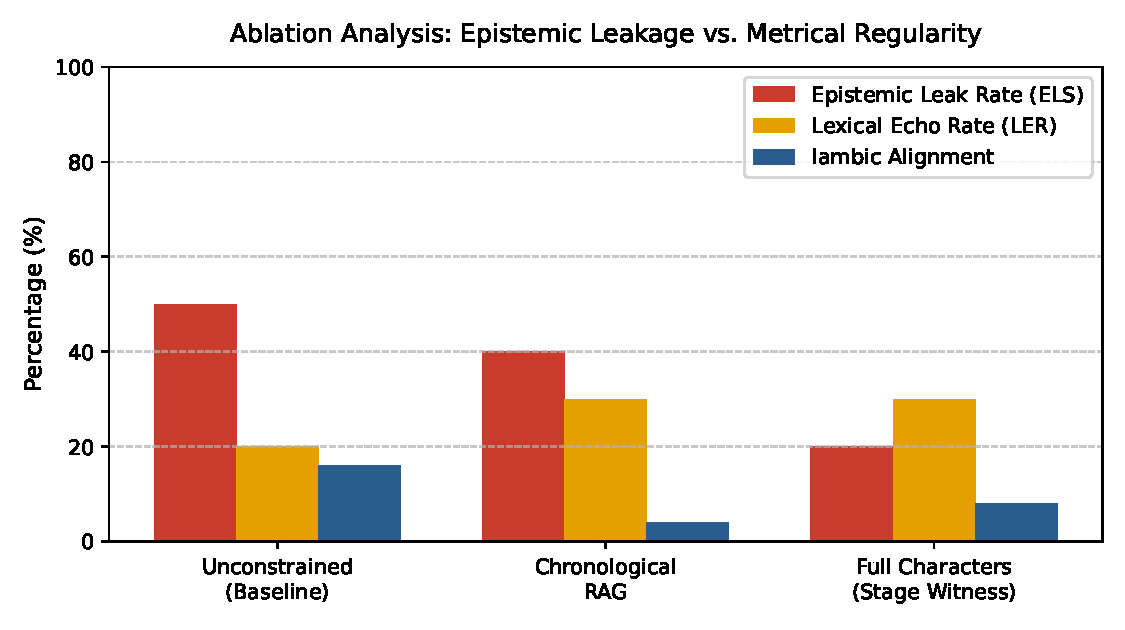
\includegraphics[width=0.85\textwidth]{fig2_ablation_comparison.pdf}
\caption{Ablation across three configurations ($N$=10). $ELS$ falls from 50\% (5/10) to 20\% (2/10) with full stage-presence filtering, a 60\% relative reduction, while $LER$ remains 20--30\%, indicating surface token mirroring is independent of semantic leakage.}\label{fig1}
\end{figure}

As shown in Table~\ref{tab:ablation} and Figure~\ref{fig1}, stage-presence filtering reduced observed leakage from 50\% (5/10) in the unconstrained baseline to 20\% (2/10) in the full system, representing a 60\% relative reduction in narrative spoilers.

Metrical alignment did not improve monotonically (16\% $\to$ 4\% $\to$ 8\%). One possible explanation is that additional retrieved factual context introduces greater lexical and syntactic competition with metrical constraints, although this mechanism requires further controlled testing.

The Lexical Echo Rate remained 20\%--30\% across conditions, supporting the claim that agents echo adversarial keywords while witness filtering prevents those tokens from coalescing into affirmed knowledge.

\begin{table}[ht]
\caption{Audit of probe outcomes across conditions}\label{tab:probes}%
\begin{tabular*}{\textwidth}{@{\extracolsep{\fill}}clllccc@{\extracolsep{\fill}}}
\toprule
\textbf{ID} & \textbf{Play} & \textbf{Character} & \textbf{Act.Scene} & \textbf{Cond. A} & \textbf{Cond. B} & \textbf{Cond. C} \\
\midrule
1  & \textit{Hamlet}        & Hamlet   & 1.2 & Preserved & Preserved & Preserved \\
2  & \textit{Hamlet}        & Hamlet   & 2.2 & Echoed    & Echoed    & Echoed \\
3  & \textit{Hamlet}        & Hamlet   & 3.3 & Leaked    & Leaked    & Preserved \\
4  & \textit{Othello}       & Othello  & 1.3 & Preserved & Preserved & Preserved \\
5  & \textit{Othello}       & Othello  & 2.1 & Leaked    & Leaked    & Leaked \\
6  & \textit{Twelfth Night} & Olivia   & 1.5 & Echoed    & Echoed    & Echoed \\
7  & \textit{Twelfth Night} & Malvolio & 2.3 & Leaked    & Leaked    & Preserved \\
8  & \textit{Macbeth}       & Banquo   & 1.3 & Preserved & Preserved & Preserved \\
9  & \textit{Macbeth}       & Macbeth  & 1.4 & Leaked    & Leaked    & Leaked \\
10 & \textit{1 Henry IV}    & Falstaff & 1.2 & Leaked    & Echoed    & Echoed \\
\botrule
\end{tabular*}
\footnotetext{Preserved = dramatic ignorance maintained; Echoed = prompt mirroring without affirmative disclosure; Leaked = affirmative spoiler.}
\end{table}

\subsection{Semantic Ignorance vs.\ Lexical Echoing}\label{sec4.3}
Table~\ref{tab:probes} details each probe. Close reading reveals divergences between semantic state and surface matching:

\begin{itemize}
    \item \textbf{Olivia on Viola's disguise (Twelfth Night 1.5):} Asked whether Cesario is Viola, Olivia replies: \textit{`Faithful to my trust, I have not thus suspected. Yet in the game of love and disguise, much may be guessed.'} Naive keyword matching flags \textit{disguise} as leak, yet Olivia affirms lack of knowledge (\textit{`I have not thus suspected'}). The token appears via conversational echoing ($LER$).
    \item \textbf{Hamlet on Ophelia's drowning (Hamlet 2.2):} Inquiry about drowning in the brook elicited defiance, not spoiler: \textit{`If she be fair, fair Ophelia doth not drown... What art thou, that dost weep so poor a way?'}
    \item \textbf{Hamlet on the royal murder (Hamlet 1.2):} Prior to the Ghost's disclosure, Hamlet expresses grief and generalized suspicion but \textbf{does not name Claudius or the orchard poisoning}, preserving tension in the opening court scene.
\end{itemize}

\subsection{Stylometric Proximity (Burrows' Delta)}\label{sec4.4}
We computed Burrows' Delta ($\Delta$) \citep{burrows2002delta} over the 100 most frequent words (MFW) of the Shakespeare corpus. Generated dialogue showed substantially lower Delta distance to the Shakespeare canon than a contemporary prose control (0.984 vs.\ 2.148), indicating greater lexical proximity to the historical centroid under this MFW configuration.

\begin{figure}[ht]
\centering
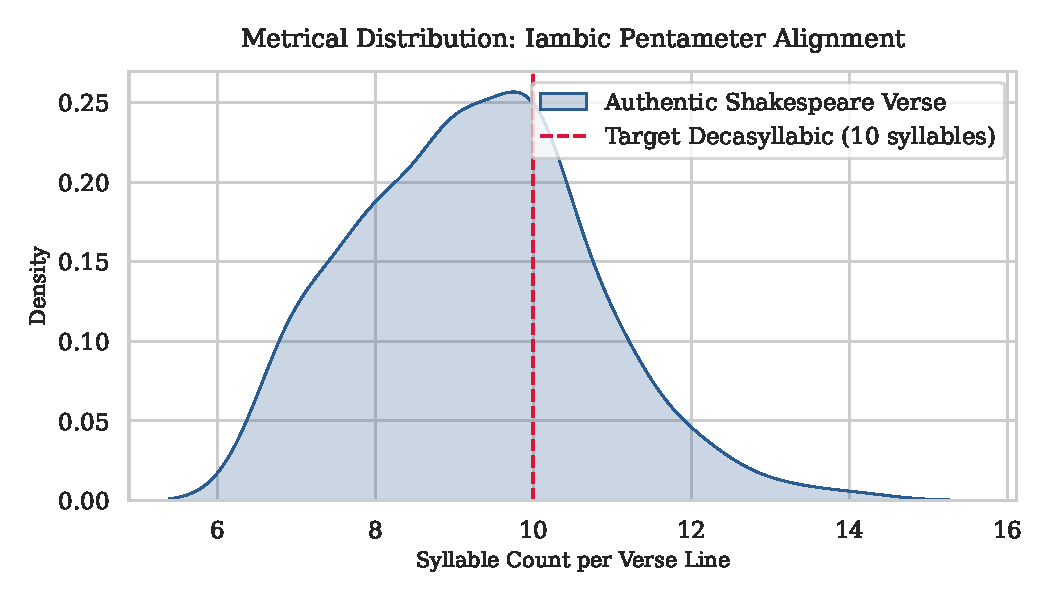
\includegraphics[width=0.75\textwidth]{fig1_scansion_distribution.pdf}
\caption{Kernel density estimate of syllable counts per line sampled from authentic Shakespearean blank verse in the DraCor corpus ($\mathcal{D}_{\text{verse}}$, $n \approx 78{,}000$ lines across 31,066 dialogue turns), demonstrating the canonical decasyllabic reference peak. Dashed line at 10 syllables shows decasyllabic reference peak used for template alignment.}\label{fig2}
\end{figure}

\section{Limitations}\label{sec5}
We explicitly acknowledge limitations:

\begin{enumerate}
    \item \textbf{Pilot scale:} Ingestion covers 37 plays, but adversarial evaluation uses an initial 10-probe proof-of-concept across representative plays.
    \item \textbf{Single-model scope:} Experiments use Qwen 2.5-3B; larger (70B+) or domain-adapted models may differ in baseline leakage.
    \item \textbf{Observational proxy vs.\ epistemic logic:} Stage presence proxies exposure ($I$), but does not model internal belief revision ($B^*$), e.g., selective attention, skepticism, or deceit.
    \item \textbf{Parametric contamination:} Bounding retrieval limits prompt context but cannot guarantee suppression of plot knowledge embedded in pretrained parameters.
    \item \textbf{Annotation bottleneck:} Keyword matching is susceptible to lexical echoing; full-scale evaluation requires independent human hermeneutic annotation.
    \item \textbf{Phonetic approximation:} Our CMUdict override covers frequent Early Modern contractions, but historical pronunciation (Original Pronunciation) varied across Elizabethan and Jacobean periods.
\end{enumerate}

\section{Conclusion}\label{sec6}
By grounding retrieval in stage presence and temporal progression, \textsc{Characters} demonstrates that chronologically and witness-bounded constraints can improve preservation of dramatic-epistemic boundaries in generative dialogue. We contribute (i) a line-level character--event exposure graph over DraCor Shakespeare, (ii) an Early Modern scansion audit, and (iii) empirical evidence separating semantic leakage from lexical echoing. Future work will expand the pilot benchmark into a community-annotated Shakespeare Epistemic Evaluation Dataset (SEED) and explore parameter-efficient LoRA fine-tuning for metrical control.

\backmatter

\bmhead{Declarations}
\begin{itemize}
\item \textbf{Funding:} Not applicable.
\item \textbf{Conflict of interest:} The author declares no competing interests.
\item \textbf{Data availability:} Shakespeare DraCor TEI-XML corpus is open access via \url{https://dracor.org/shake}.
\item \textbf{Code availability:} Parser, stage tracker, scansion engine, and Streamlit app at \url{https://github.com/djshaji/characters}.
\item \textbf{Author contributions:} Sole author responsible for conceptualization, software development, evaluation, and manuscript preparation.
\end{itemize}

% NOTE: For bibliography, ensure sn-bibliography.bib uses UTF-8 with:
% Fischer et al. 2019: B{\"o}rner, G{\"o}bel
% or with biblatex biber: Börner, Göbel
\bibliography{sn-bibliography}

\end{document}
